\section{Experimental Set-up}
\label{sec:setup}

The investigated $LaBr_3(Ce)$ detectors are cylindrical crystals of 9.8 cm diameter aligned at 180° in front of each other (fig. \ref{fig:setup}). The detectors are coupled with photomultipliers powered at 690-650 V. The output of the PMTs is directly read by a CAEN DT5730 digitizer equipped with DPP-PSD firmware, read in turn by the CoMPASS software. Henceforth, we will distinguish the two detectors by referring to them as \emph{channel 0} and \emph{channel 1}. \\

The radioactive sources used are: Cobalt-60, Cesium-137 and Sodium-22. The samples' actvities are 376 kBq, 389 kBq and 418 kBq respectively, with an error of 3\%. The samples are located in the middle of the two detectors. 
For each sample, a run is recorded at each of the following distances: 10 cm, 15 cm and 20 cm. An additional run, for a total of 10, is taken without any source to record the internal background.
	
\begin{figure}[h!]
\centering
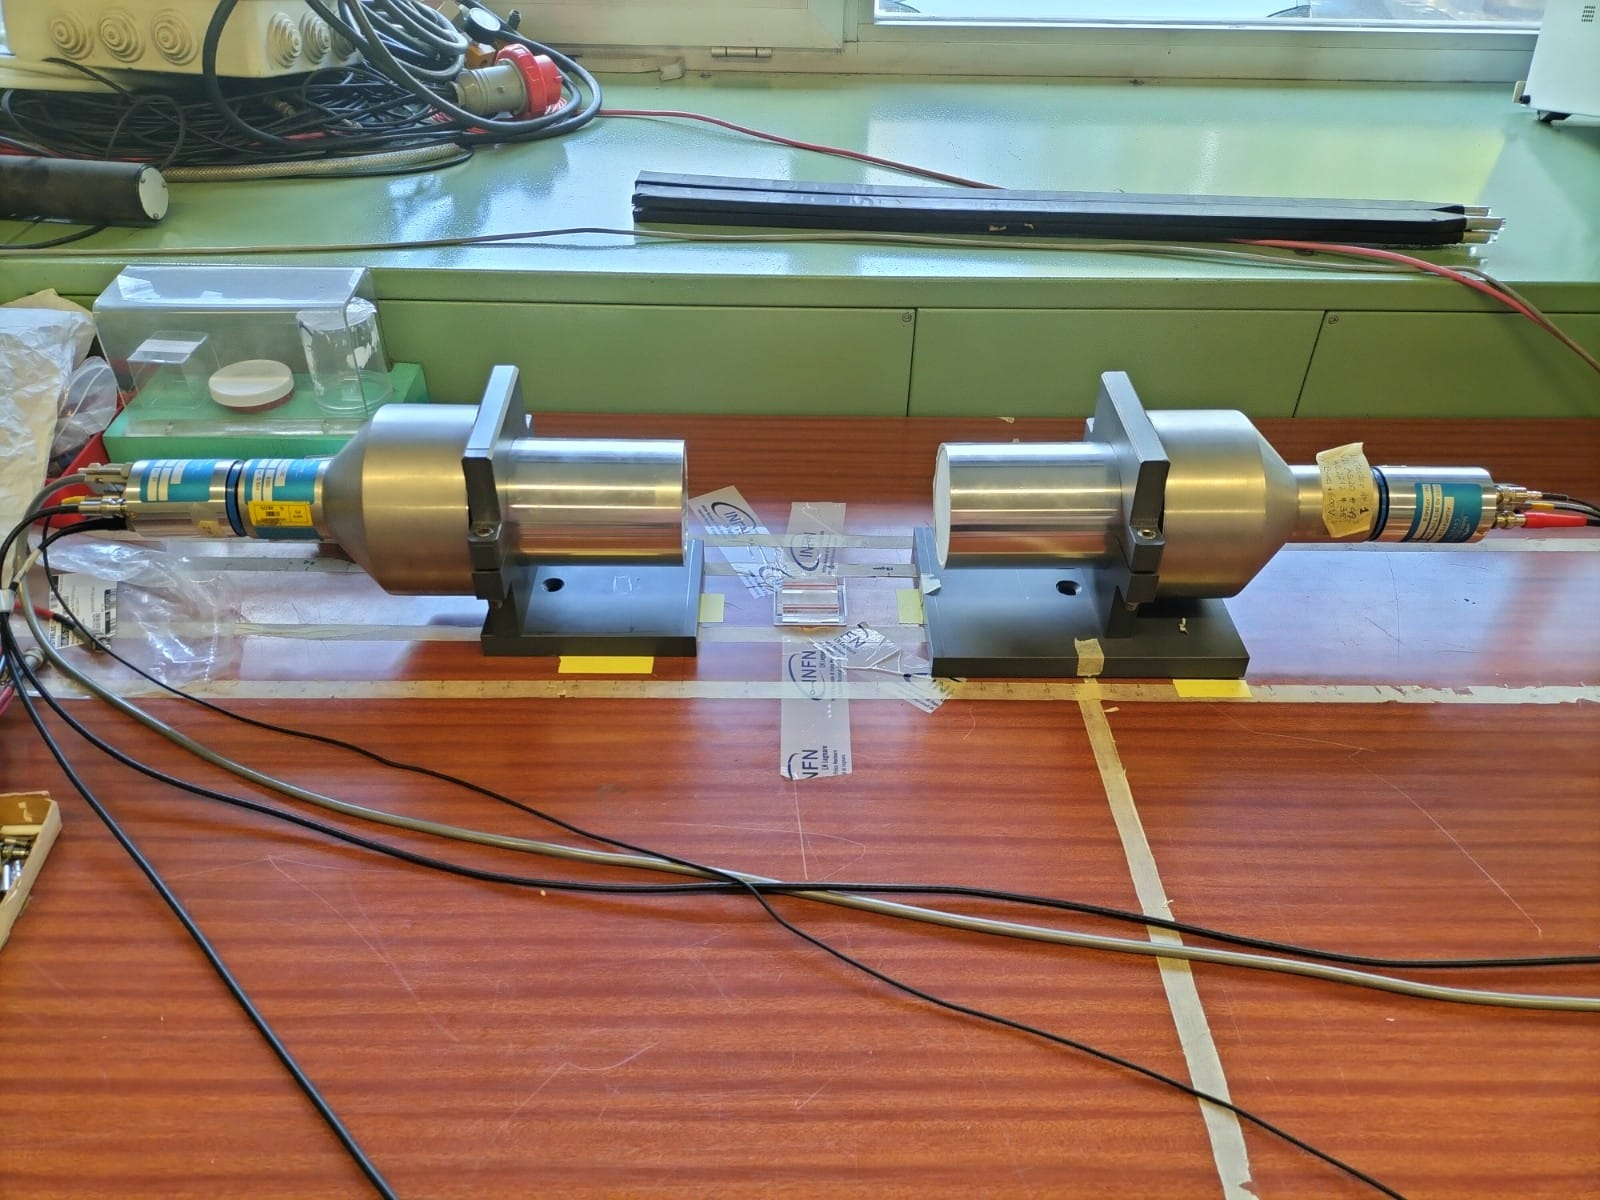
\includegraphics[width=0.6\textwidth]{Images/lab/Calibration.jpeg}
\caption{Photo of the detector set-up.}
\label{fig:setup}
\end{figure}